\chapter{Modelos convexos}
\label{cap:convexos}

Este capítulo aplica la teoría del Capítulo~\ref{cap:optimizacion} a dos modelos cuyo entrenamiento es un problema
convexo: la regresión logística y la máquina de vectores soporte (SVM). Se presentan sus resultados en Bonn y en
CHB-MIT y se verifican numéricamente tres afirmaciones teóricas: que la logística tiene un único óptimo global al que
se llega desde cualquier punto inicial, que una red neuronal chica no lo tiene, y que el SVM cumple las condiciones
KKT con brecha de dualidad nula. Todo el código está en el notebook \texttt{etapa3\_modelos\_clasicos.ipynb}.

\section{Regresión logística}
\label{sec:logistica}

\subsection{Modelo multinomial}

Con $K$ clases y atributos $\vx \in \R^d$, el modelo calcula un puntaje lineal por clase y lo lleva al simplex con la
función softmax (Sección~\ref{sec:softmax}):
\begin{equation}
  z_k = \vw_k^\top\vx + b_k, \qquad P(y = k \mid \vx) = p_k(\vx) = \frac{e^{z_k}}{\sum_j e^{z_j}}.
\end{equation}
Se entrena minimizando la entropía cruzada (el negativo de la log-verosimilitud) más una penalización L2:
\begin{equation}
  J(W, \mathbf{b}) = -\frac1n\sum_{i=1}^n\log p_{y_i}(\vx_i) + \frac{\lambda}{2}\lVert W\rVert_F^2.
  \label{eq:ce_multinomial}
\end{equation}
Por~\eqref{eq:grad_ce}, el gradiente respecto de $\vw_k$ es $\frac1n\sum_i (p_{ik} - \mathds{1}[y_i = k])\,\vx_i + \lambda\vw_k$:
el error de predicción ponderado por los atributos. En \texttt{scikit-learn} la regularización se expresa con
$C = 1/(\lambda n)$.

\subsection{Caso binario: convexidad estricta}

Para dos clases, con $y_i \in \{0, 1\}$, $\vth = (\vw, b)$, $\tilde\vx_i = (\vx_i, 1)$ y $\sigma(z) = 1/(1 + e^{-z})$,
\begin{equation}
  J(\vth) = \frac1n\sum_{i=1}^n\Big[\log\big(1 + e^{\vth^\top\tilde\vx_i}\big) - y_i\,\vth^\top\tilde\vx_i\Big] + \frac{\lambda}{2}\lVert\vw\rVert^2.
  \label{eq:logistica_binaria}
\end{equation}

\begin{proposicion}
\label{prop:logistica_convexa}
Sea $p_i = \sigma(\vth^\top\tilde\vx_i)$, $S = \operatorname{diag}\big(p_i(1 - p_i)\big)$ y $\tilde X$ la matriz con filas $\tilde\vx_i^\top$.
Entonces
\begin{equation}
  \nabla J(\vth) = \frac1n\tilde X^\top(\mathbf{p} - \mathbf{y}) + \lambda\begin{pmatrix}\vw\\0\end{pmatrix},
  \qquad
  \nabla^2 J(\vth) = \frac1n\tilde X^\top S\,\tilde X + \lambda\begin{pmatrix}I & 0\\0 & 0\end{pmatrix}.
  \label{eq:hess_logistica}
\end{equation}
Si $\tilde X$ tiene rango completo, $\nabla^2 J(\vth) \succ 0$ en todo $\vth$: $J$ es estrictamente convexa y tiene a lo
sumo un minimizador. Además $\nabla J$ es Lipschitz con constante
\begin{equation}
  L \le \frac{1}{4n}\lambda_{\max}\big(\tilde X^\top\tilde X\big) + \lambda.
  \label{eq:L_logistica}
\end{equation}
\end{proposicion}
\begin{proof}
Con $z = \vth^\top\tilde\vx_i$, $\frac{d}{dz}\log(1 + e^z) = \sigma(z)$ y $\sigma'(z) = \sigma(z)(1 - \sigma(z))$. Por la regla
de la cadena, el gradiente del término $i$ es $(p_i - y_i)\tilde\vx_i$ y su Hessiana es $p_i(1 - p_i)\,\tilde\vx_i\tilde\vx_i^\top$;
sumando se obtiene~\eqref{eq:hess_logistica}. Para $\mathbf{v} = (\mathbf{v}_w, v_b) \neq \mathbf{0}$,
\[
  \mathbf{v}^\top\nabla^2 J\,\mathbf{v} = \frac1n\big\lVert S^{1/2}\tilde X\mathbf{v}\big\rVert^2 + \lambda\lVert\mathbf{v}_w\rVert^2 > 0,
\]
porque $p_i(1 - p_i) > 0$ y $\tilde X\mathbf{v} \neq \mathbf{0}$ por el rango completo. La unicidad sale del
Teorema~\ref{teo:local_global}. Para la cota, $p_i(1 - p_i) \le \frac14$ implica
$\nabla^2 J \preceq \frac{1}{4n}\tilde X^\top\tilde X + \lambda I$, cuyo mayor autovalor es la cota~\eqref{eq:L_logistica}.
\end{proof}

La consecuencia práctica es fuerte: el resultado del entrenamiento no depende ni del punto inicial ni del algoritmo,
siempre que converja. Cualquier diferencia entre dos implementaciones es un problema de convergencia, no un óptimo
distinto. Con la cota~\eqref{eq:L_logistica} el descenso por gradiente con paso $1/L$ converge desde cualquier punto
(Teorema~\ref{teo:convergencia}).

\paragraph{Separabilidad.} Sin regularización ($\lambda = 0$), si las clases son linealmente separables el mínimo no
existe: multiplicar $\vth$ por una constante cada vez mayor sigue bajando la pérdida hacia 0. La penalización L2 lo
evita, porque la vuelve fuertemente convexa en $\vw$ y garantiza que el mínimo existe. En Bonn el problema ictal contra
el resto es casi separable, así que esto no es una sutileza.

\section{Máquinas de vectores soporte}
\label{sec:svm}

El SVM de margen blando, su dual y las condiciones KKT se dedujeron en la Sección~\ref{sec:svm_dual}. Escrito sin
restricciones, el primal~\eqref{eq:svm_primal} es
\begin{equation}
  \min_{\vw, b}\ \frac12\lVert\vw\rVert^2 + C\sum_i\max\big(0,\ 1 - y_i(\vw^\top\vx_i + b)\big),
\end{equation}
la pérdida \emph{bisagra} más una penalización L2. Comparada con la logística, la bisagra es exactamente cero para los
puntos bien clasificados con margen, mientras que $\log(1 + e^{-m})$ es positiva para todo margen $m$: por eso en el SVM
solo influyen los vectores soporte. A cambio, la bisagra no es diferenciable en $m = 1$ y el SVM no da probabilidades.

Se usan tres variantes: SVM lineal y SVM con núcleo RBF en Bonn (\texttt{SVC}, que resuelve el dual con el algoritmo SMO),
y SVM lineal en CHB-MIT (\texttt{LinearSVC} resolviendo el primal, mucho más rápido con 200\,000 ventanas).

\section{Configuración experimental}

\begin{itemize}
  \item \textbf{Atributos:} log-potencia de Welch. Bonn: 20 bandas de 2~Hz entre 0,5 y 40~Hz. CHB-MIT: 18 canales
        $\times$ 5 bandas. En ambos casos se estandarizan (media 0, desvío 1) con los datos de entrenamiento de cada
        partición.
  \item \textbf{Bonn:} logística con $C = 1$; SVM lineal con $C = 1$; SVM RBF con $C = 10$ y
        $\gamma = 1/(d\cdot\operatorname{Var}(\vx))$. Validación cruzada estratificada $10\times5$.
  \item \textbf{CHB-MIT:} logística con $C = 0{,}1$ y SVM lineal con $C = 0{,}01$, ambos con peso de clases balanceado
        (cada clase pesa en la pérdida en proporción inversa a su frecuencia). Ventanas de borde excluidas del
        entrenamiento. Suavizado causal de 3 ventanas y umbral de Neyman-Pearson con $\alpha = 10^{-3}$.
\end{itemize}

\section{Resultados en Bonn}
\label{sec:bonn_resultados}

\subsection{Desempeño}

\begin{table}[ht]
\centering
\caption{Bonn, 3 clases: validación cruzada estratificada de 10 particiones repetida 5 veces (media $\pm$ desvío sobre
las 50 particiones).}
\label{tab:bonn_cv}
\begin{tabular}{lccc}
\toprule
Modelo & Exactitud & Exactitud balanceada & $F_1$ macro \\
\midrule
Regresión logística & $0{,}974 \pm 0{,}018$ & $0{,}972 \pm 0{,}022$ & $0{,}972 \pm 0{,}020$ \\
SVM lineal          & $0{,}973 \pm 0{,}020$ & $0{,}968 \pm 0{,}027$ & $0{,}970 \pm 0{,}024$ \\
SVM RBF             & $\mathbf{0{,}984 \pm 0{,}016}$ & $\mathbf{0{,}981 \pm 0{,}019}$ & $\mathbf{0{,}982 \pm 0{,}018}$ \\
\bottomrule
\end{tabular}
\end{table}

\begin{table}[ht]
\centering
\caption{Bonn: sensibilidad, especificidad y AUC de cada clase contra el resto (predicciones fuera de la partición,
validación cruzada de 10 particiones).}
\label{tab:bonn_clases}
\begin{tabular}{llccc}
\toprule
Modelo & Clase & Sensibilidad & Especificidad & AUC \\
\midrule
\multirow{3}{*}{Logística}
 & sano       & 0,990 & 0,990 & 0,999 \\
 & interictal & 0,970 & 0,983 & 0,998 \\
 & ictal      & 0,960 & 0,990 & 0,998 \\
\midrule
\multirow{3}{*}{SVM lineal}
 & sano       & 0,990 & 0,993 & 0,993 \\
 & interictal & 0,970 & 0,980 & 0,994 \\
 & ictal      & 0,960 & 0,990 & 0,993 \\
\midrule
\multirow{3}{*}{SVM RBF}
 & sano       & 0,995 & 0,997 & 0,999 \\
 & interictal & 0,985 & 0,987 & 0,998 \\
 & ictal      & 0,970 & 0,995 & 0,995 \\
\bottomrule
\end{tabular}
\end{table}

Con solo 20 atributos espectrales, un modelo lineal clasifica bien el 97~\% de los segmentos (Tablas~\ref{tab:bonn_cv}
y~\ref{tab:bonn_clases}). El núcleo RBF agrega un punto. La clase con menor sensibilidad es la ictal, y las matrices
de confusión (Figura~\ref{fig:bonn_confusion}) muestran que los errores se concentran entre interictal e ictal: algunos
segmentos del foco epileptógeno (set D) tienen actividad parecida a una crisis. Un segmento sano casi nunca se confunde
con uno ictal. Las curvas ROC (Figura~\ref{fig:bonn_roc}) están pegadas a la esquina superior izquierda, con AUC entre
0,993 y 0,999.

Estos números son altos pero optimistas, por las razones de la Sección~\ref{sec:bonn}: no se separa por paciente y los
segmentos se eligieron sin artefactos.

\begin{figure}[ht]
  \centering
  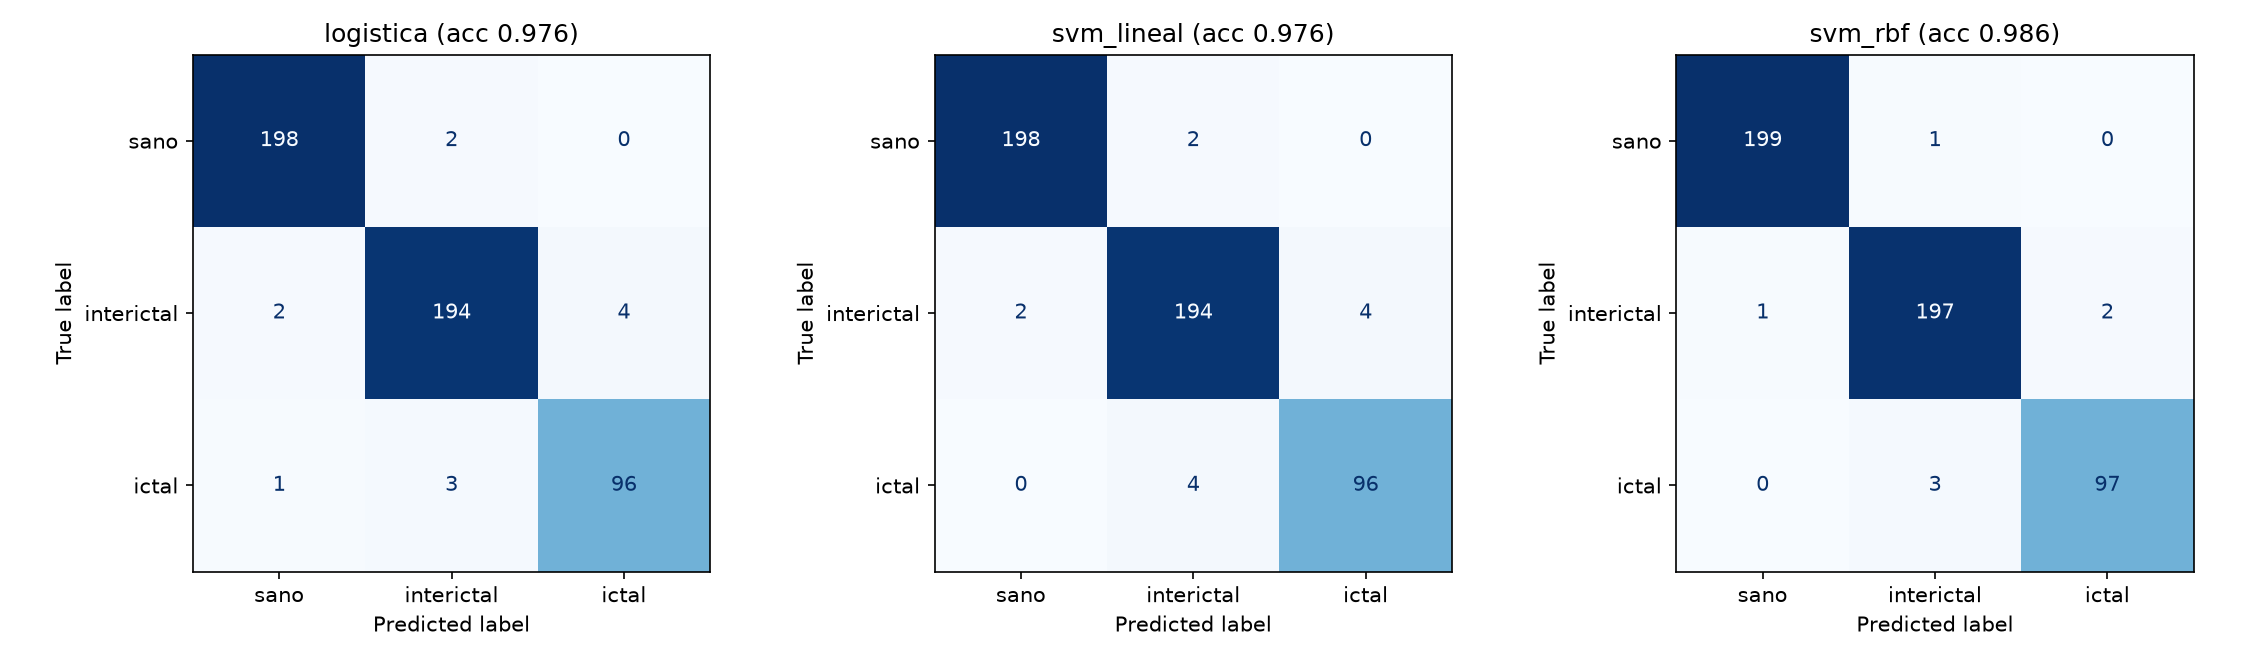
\includegraphics[width=\textwidth]{etapa3/bonn_matrices_confusion.png}
  \caption{Bonn: matrices de confusión con predicciones fuera de la partición (validación cruzada de 10 particiones).}
  \label{fig:bonn_confusion}
\end{figure}

\begin{figure}[ht]
  \centering
  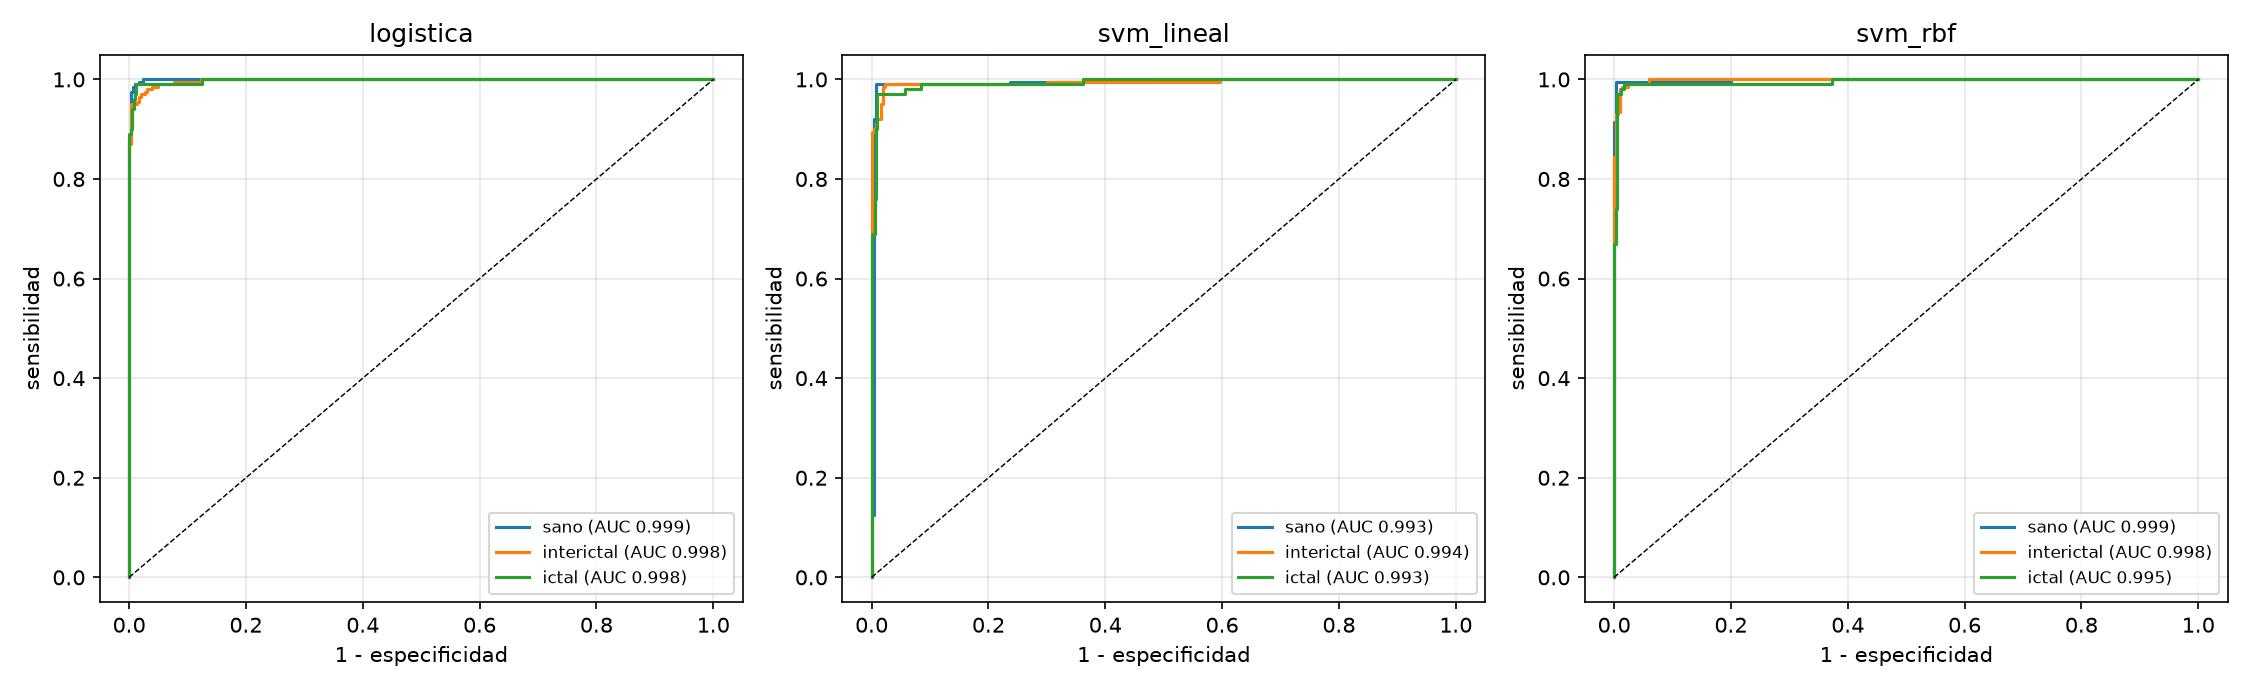
\includegraphics[width=\textwidth]{etapa3/bonn_roc.png}
  \caption{Bonn: curvas ROC de cada clase contra el resto.}
  \label{fig:bonn_roc}
\end{figure}

\subsection{Las probabilidades sobre el simplex}

Cada segmento recibe un vector $\mathbf{p} = (p_\text{sano}, p_\text{interictal}, p_\text{ictal}) \in \Delta^2$, un punto del
triángulo de la Figura~\ref{fig:simplex_teorico}. Para graficarlo en el plano se usan las coordenadas
$u = p_2 + p_3/2$, $v = \frac{\sqrt3}{2}p_3$, que llevan los vértices a $(0,0)$, $(1,0)$ y $(\frac12, \frac{\sqrt3}{2})$.

\begin{figure}[ht]
  \centering
  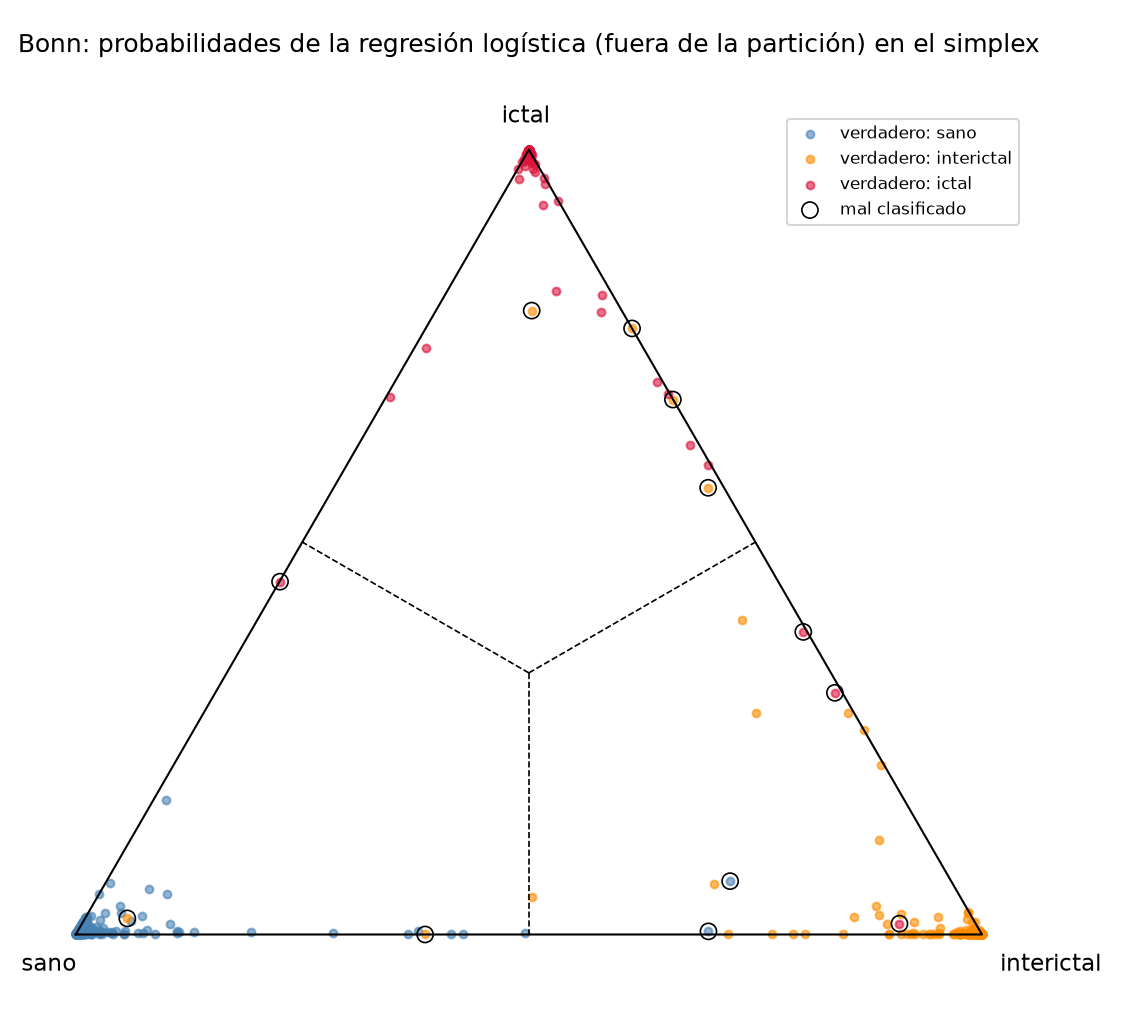
\includegraphics[width=0.75\textwidth]{etapa3/bonn_simplex.png}
  \caption{Bonn: probabilidades de la regresión logística (fuera de la partición) sobre el simplex $\Delta^2$. Las líneas
           punteadas son las fronteras de la regla $\argmax$; los círculos negros, los segmentos mal clasificados.}
  \label{fig:bonn_simplex}
\end{figure}

La Figura~\ref{fig:bonn_simplex} muestra que casi todos los segmentos quedan pegados a su vértice: el modelo predice con
mucha certeza. Los errores están sobre el lado ictal--interictal del triángulo, donde la probabilidad de ``sano'' es
casi cero: el modelo no duda entre las tres clases, duda entre dos. Algunos segmentos sanos caen sobre el lado
sano--interictal. No se verificó de qué set son; una explicación posible es la potencia alfa del set B (ojos cerrados),
que podría acercarlos a algunos registros intracraneales.

\subsection{Qué frecuencias usa el modelo}

Con atributos estandarizados, el coeficiente $w_{k,j}$ indica cuánto aumenta el puntaje de la clase $k$ si la
log-potencia de la banda $j$ sube un desvío estándar (Figura~\ref{fig:bonn_coef}).

\begin{figure}[ht]
  \centering
  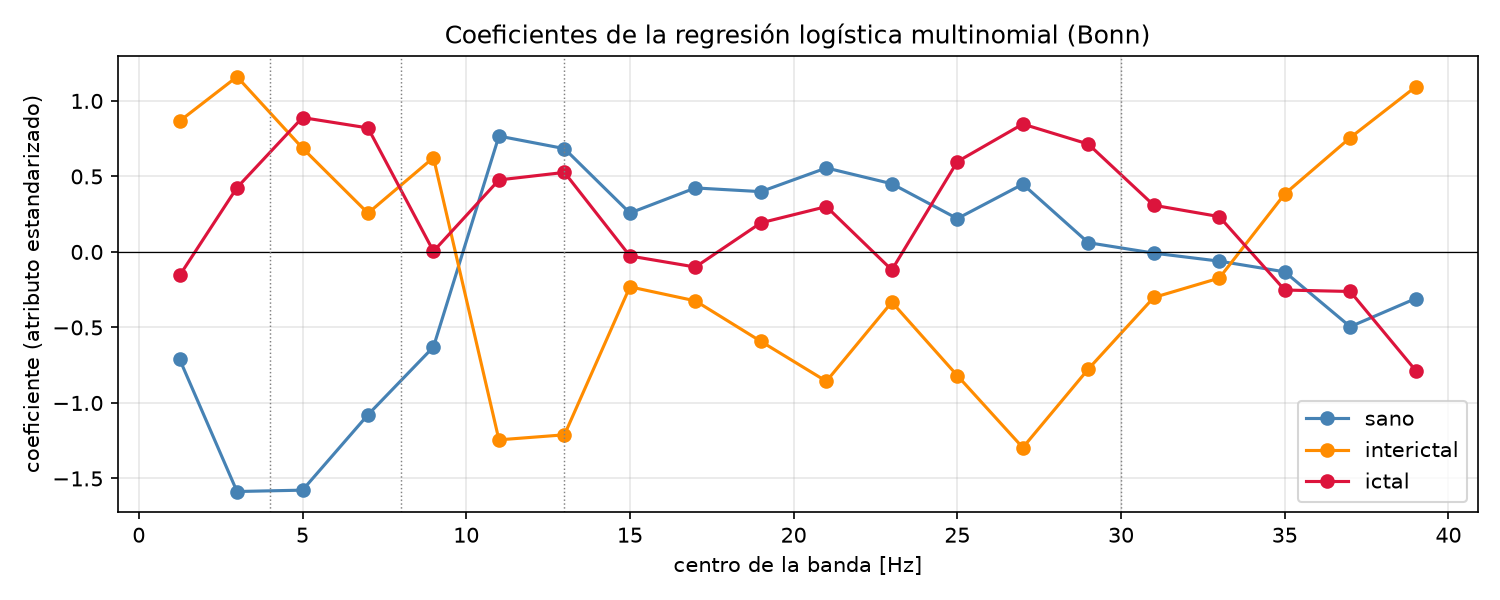
\includegraphics[width=0.9\textwidth]{etapa3/bonn_coeficientes.png}
  \caption{Coeficientes de la regresión logística multinomial en Bonn, por banda de 2~Hz. Las líneas verticales marcan
           los límites de las bandas clínicas (4, 8, 13 y 30~Hz).}
  \label{fig:bonn_coef}
\end{figure}

\begin{itemize}
  \item \textbf{Sano:} coeficientes negativos grandes entre 2 y 8~Hz ($-1{,}6$) y positivos entre 10 y 30~Hz. El EEG de
        superficie de voluntarios sanos tiene relativamente poca actividad lenta y más alfa y beta.
  \item \textbf{Interictal:} el patrón opuesto: positivo en delta (hasta $+1{,}2$ en 2--4~Hz) y negativo en alfa y beta.
        Coincide con la Tabla~\ref{tab:bonn_bandas}, donde los sets C y D tienen 60--67~\% de su potencia en delta.
        También es positivo entre 36 y 40~Hz, probablemente por diferencias del equipo intracraneal.
  \item \textbf{Ictal:} positivo en theta (4--8~Hz, $+0{,}9$), donde está la descarga rítmica, y en beta alta (24--30~Hz).
\end{itemize}
Como softmax es invariante a sumar el mismo vector a los tres $\vw_k$, solo importan las diferencias entre clases: los
coeficientes individuales se interpretan con cuidado.

\section{Verificación de la optimalidad global}
\label{sec:verif_optimalidad}

\subsection{Regresión logística: 20 puntos iniciales, un solo óptimo}

Se toma el problema binario ictal contra el resto en Bonn, con 20 atributos estandarizados más el sesgo y $\lambda = 0{,}01$,
y se implementa el descenso por gradiente a mano con el gradiente~\eqref{eq:hess_logistica} y el paso $\eta = 1/L$ de
la cota~\eqref{eq:L_logistica}: $L = 4{,}298$, $\eta = 0{,}233$. Se corren 20\,000 iteraciones desde 20 puntos
iniciales $\vth_0 \sim \mathcal{N}(\mathbf{0}, 9I)$, que quedan a una distancia media de 13,2 del óptimo. Como
referencia se usa la solución de \texttt{scikit-learn} con tolerancia $10^{-12}$, de valor $J^* = 0{,}07699786$.

Resultados:
\begin{itemize}
  \item Los 20 valores finales de $J$ coinciden con $J^*$ en las 8 cifras informadas.
  \item La mayor distancia entre un $\vth$ final y el de referencia es $3{,}0\times10^{-7}$.
  \item La brecha $J(\vth_k) - J^*$ cae en línea recta en escala logarítmica (Figura~\ref{fig:optimalidad}, izquierda):
        convergencia lineal, como predice el Teorema~\ref{teo:convergencia}. La curva se aplana en $10^{-16}$, la
        precisión del punto flotante de doble precisión.
\end{itemize}
La pendiente observada concuerda con la teoría. En el óptimo, el menor autovalor de la Hessiana es $\mu \approx 0{,}0081$,
lo que da $\kappa = L/\mu \approx 528$ y una tasa de $1 - 1/\kappa \approx 0{,}998$ por iteración: unas 14\,600
iteraciones para 12 órdenes de magnitud, dentro de las 20\,000 usadas. El $\kappa$ alto se debe a que $L$ es una cota
global (supone $p_i(1 - p_i) = \frac14$) mientras que cerca del óptimo casi todos los $p_i$ están cerca de 0 o 1 y la
curvatura real es mucho menor: el mayor autovalor de la Hessiana en el óptimo es 0,24, no 4,3.

\begin{figure}[ht]
  \centering
  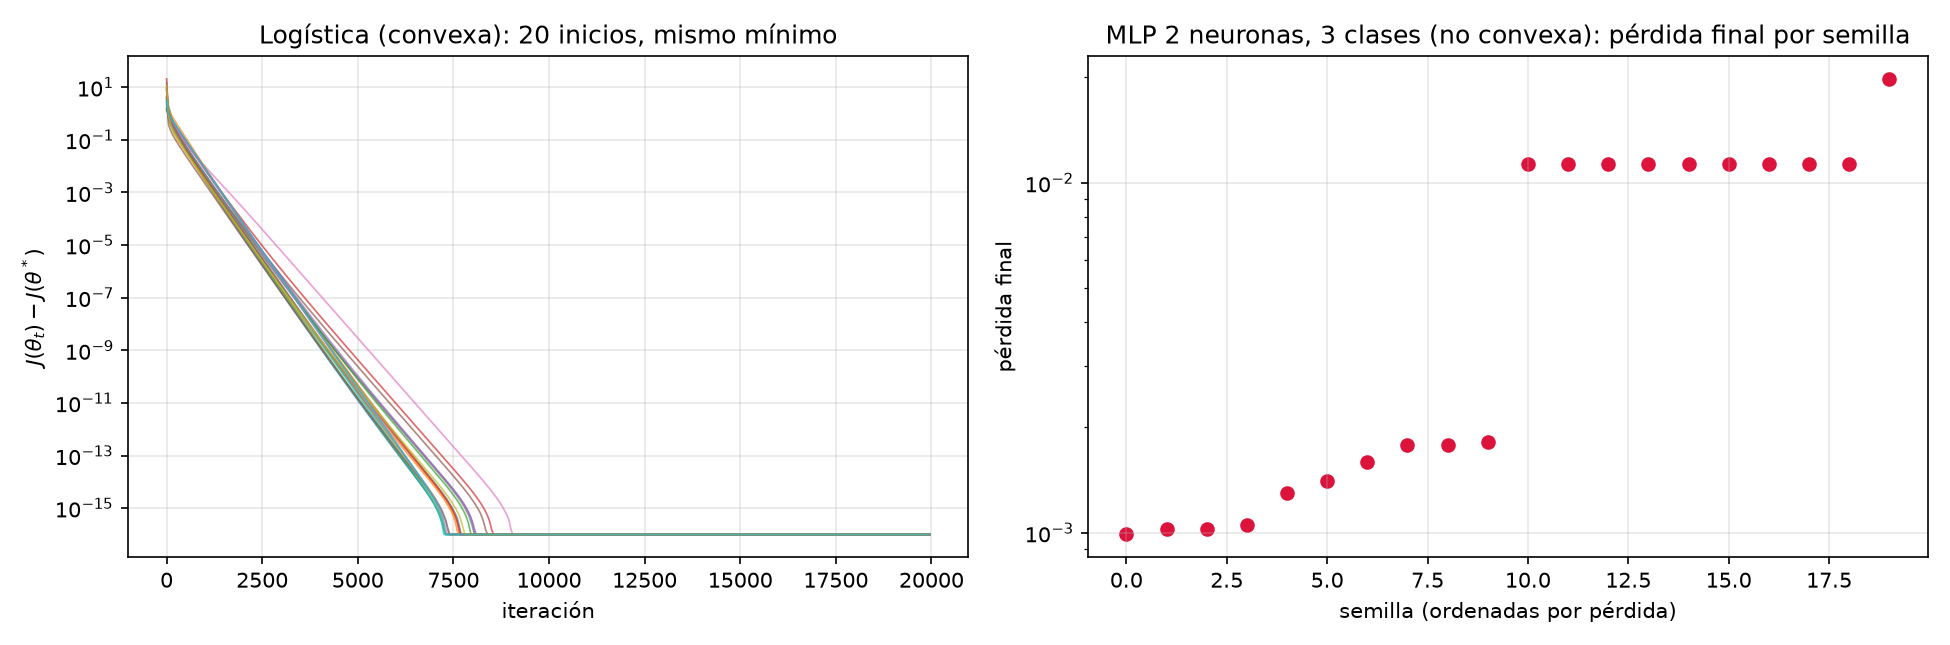
\includegraphics[width=\textwidth]{etapa3/optimalidad_convexo_vs_no_convexo.png}
  \caption{Izquierda: brecha $J(\vth_k) - J^*$ de la regresión logística (convexa) desde 20 puntos iniciales, en escala
           logarítmica. Derecha: pérdida final de un perceptrón de 2 neuronas (no convexo) con 20 semillas, ordenadas.}
  \label{fig:optimalidad}
\end{figure}

\subsection{Contraste: una red neuronal chica}

Se entrena un perceptrón multicapa con una capa oculta $\tanh$ hasta convergencia (L-BFGS, tolerancia $10^{-10}$) desde
20 semillas, en dos configuraciones.

\paragraph{(a) Ictal contra el resto, 4 neuronas, penalización $\alpha = 1$.} Las 20 semillas terminan con la \emph{misma}
pérdida, 0,041217, pero con pesos distintos: las soluciones de las semillas 6 y 14 están a distancia 9,7. En el punto
medio entre ambas, la pérdida es \textbf{0,596}, catorce veces mayor. Por el Teorema~\ref{teo:local_global}(2) eso es
imposible si la función es convexa. Son mínimos equivalentes por las simetrías de la Sección~\ref{sec:no_convexo}
(permutación de neuronas y cambios de signo), que en una función convexa no pueden existir.

\paragraph{(b) Tres clases, 2 neuronas, $\alpha = 10^{-3}$.} Aparecen \textbf{8 valores distintos} de la pérdida final, entre
0,00099 y 0,01983: un factor 20 (Figura~\ref{fig:optimalidad}, derecha). Nueve de las 20 semillas quedan en el mismo
mínimo local, con pérdida 0,01135, unas diez veces peor que el mejor. Son mínimos locales genuinos: con solo 2
neuronas, la red no puede representar bien las tres clases desde cualquier configuración inicial, y el optimizador
queda atrapado en la que le toca.

\paragraph{Consecuencia.} En un modelo convexo, una corrida alcanza. En una red neuronal el resultado depende de la
semilla, y comparar dos optimizadores con una corrida de cada uno no permite separar el efecto del optimizador del
azar de la inicialización. Por eso en el Capítulo~\ref{cap:cnn} cada configuración se corre con 5 semillas.

\section{Verificación de KKT en el SVM}
\label{sec:verif_kkt}

Se entrena un SVM lineal con $C = 1$ para separar el set E (ictal, $y = +1$) del set D (interictal del foco, $y = -1$):
200 segmentos, 20 atributos estandarizados, tolerancia $10^{-8}$. A partir de los $\alpha_i$ que devuelve el
solucionador se verifica cada condición de la Sección~\ref{sec:svm_dual} (Tabla~\ref{tab:kkt_verif}).

\begin{table}[ht]
\centering
\caption{Verificación numérica de las condiciones KKT del SVM lineal (Bonn, E contra D, $C = 1$). $m_i = y_i f(\vx_i)$.}
\label{tab:kkt_verif}
\begin{tabular}{lll}
\toprule
Condición & Teoría & Medido \\
\midrule
Estacionariedad en $\vw$ & $\vw = \sum_i\alpha_i y_i\vx_i$ & diferencia máxima $0{,}0$ \\
Estacionariedad en $b$ & $\sum_i\alpha_i y_i = 0$ & $-1{,}1\times10^{-15}$ \\
Factibilidad dual & $0 \le \alpha_i \le C$ & $\min = 0$, $\max = 1$ \\
$\alpha_i = 0$ & $m_i \ge 1$ & 180 puntos, $\min m_i = 1{,}0127$ \\
$0 < \alpha_i < C$ & $m_i = 1$ & 9 puntos, $m_i \in [1{,}0000;\ 1{,}0000]$ \\
$\alpha_i = C$ & $m_i \le 1$ & 11 puntos, $\max m_i = 0{,}6293$ \\
Valor primal & & 11,692841 \\
Valor dual & & 11,692839 \\
Brecha relativa & $0$ (Slater) & $1{,}55\times10^{-7}$ \\
\bottomrule
\end{tabular}
\end{table}

\begin{figure}[ht]
  \centering
  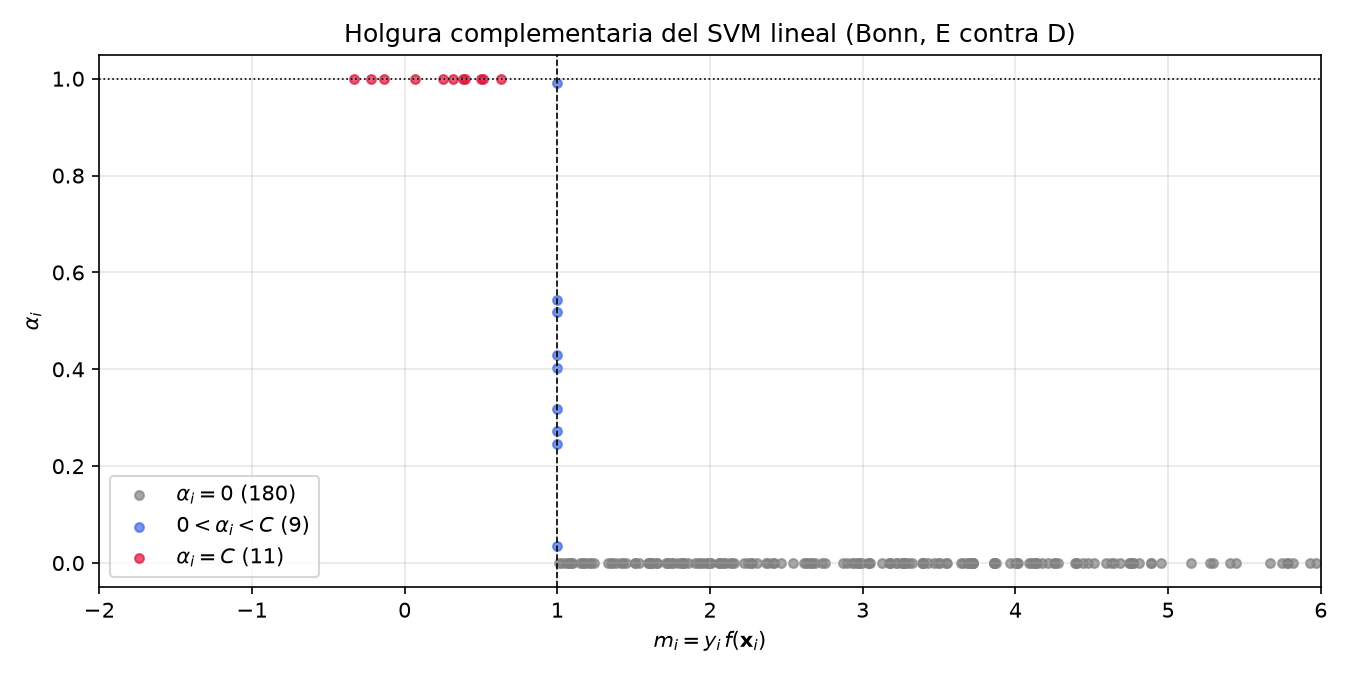
\includegraphics[width=0.85\textwidth]{etapa3/svm_kkt.png}
  \caption{Holgura complementaria en el SVM lineal: multiplicador $\alpha_i$ contra margen funcional $m_i$. Los puntos con
           $\alpha_i = 0$ están a la derecha de $m = 1$; los libres, sobre $m = 1$; los acotados en $C$, a la izquierda.}
  \label{fig:svm_kkt}
\end{figure}

Todas las condiciones se cumplen a la precisión numérica. La Figura~\ref{fig:svm_kkt} muestra la holgura complementaria:
ningún punto está en las zonas prohibidas ($\alpha_i > 0$ con $m_i > 1$, o $\alpha_i < C$ con $m_i < 1$). De los 200
segmentos solo 20 tienen $\alpha_i > 0$: el hiperplano queda determinado por esos 20 vectores soporte, y los otros 180
se podrían borrar sin que cambie la solución. De los 20, 11 están dentro del margen o mal clasificados
($\alpha_i = C$). La brecha entre primal y dual es del orden de la tolerancia del solucionador: hay dualidad fuerte,
como garantiza la condición de Slater.

\section{Resultados en CHB-MIT: paciente nuevo (LOPO)}
\label{sec:lopo}

\subsection{Resumen}

La Tabla~\ref{tab:lopo_resumen} resume los resultados de dejar un paciente fuera, sumando las 34 crisis de los 6
pacientes de prueba. Se comparan dos variantes de atributos (\emph{global}: sin calibrar; \emph{calibrado}: restando la
mediana del paciente, Sección~\ref{sec:calibracion}) y dos reglas de umbral (cero, que corresponde a $p = 0{,}5$ con
clases balanceadas, y Neyman-Pearson con $\alpha = 10^{-3}$).

\begin{table}[ht]
\centering
\caption{CHB-MIT, dejar un paciente fuera. AUC: media entre los 6 pacientes. Sensibilidad y especificidad por ventana:
media entre pacientes. Crisis y FA/h: totales sobre los 6 pacientes. Latencia: mediana.}
\label{tab:lopo_resumen}
\small
\begin{tabular}{lllccccccc}
\toprule
Variante & Modelo & Umbral & AUC & Sens. & Espec. & Crisis & FA/h & Lat. [s] \\
\midrule
\multirow{4}{*}{global}
 & logística & cero & 0,946 & 0,627 & 0,893 & 28/34 & 17,13 & 12,3 \\
 & logística & NP   & 0,946 & 0,363 & 0,994 & 23/34 & 2,10  & 20,0 \\
 & SVM lineal & cero & 0,944 & 0,625 & 0,890 & 28/34 & 17,23 & 12,3 \\
 & SVM lineal & NP   & 0,944 & 0,352 & 0,994 & 24/34 & 2,18  & 20,0 \\
\midrule
\multirow{4}{*}{calibrado}
 & logística & cero & 0,949 & 0,779 & 0,955 & 34/34 & 11,00 & 12,5 \\
 & logística & NP   & 0,949 & 0,334 & 0,994 & 24/34 & \textbf{1,14} & 25,3 \\
 & SVM lineal & cero & 0,948 & 0,772 & 0,953 & 34/34 & 11,30 & 12,5 \\
 & SVM lineal & NP   & 0,948 & 0,334 & 0,994 & 24/34 & 1,20  & 22,3 \\
\bottomrule
\end{tabular}
\end{table}

\paragraph{El umbral natural no sirve.} Con umbral cero y atributos calibrados se detectan las 34 crisis, pero con 11
falsas alarmas por hora: más de 250 por día. La especificidad por ventana de 0,955 parece alta, pero con 900 ventanas
por hora el 4,5~\% restante son 40 ventanas falsas por hora. Es la ilustración directa de la
Sección~\ref{sec:zona_util}.

\paragraph{Neyman-Pearson.} Con $\alpha = 10^{-3}$ las falsas alarmas bajan diez veces, a 1,1--2,2 por hora, a cambio de
detectar el 70~\% de las crisis y de duplicar la latencia. Es el compromiso sensibilidad--especificidad resuelto
explícitamente con un multiplicador de Lagrange.

\paragraph{Calibrar.} Con la misma sensibilidad por evento (24/34), restar la mediana del paciente baja las falsas alarmas
casi a la mitad (de 2,10 a 1,14 por hora con la logística). Confirma que buena parte de la dificultad de generalizar a un
paciente nuevo es la diferencia de nivel basal, el término $2\log g_{p,c}$ del modelo.

\paragraph{Logística contra SVM.} Los resultados son casi idénticos. Ambos son clasificadores lineales sobre los mismos
atributos; solo cambia la pérdida (logística contra bisagra), y con miles de ejemplos la frontera resultante es muy
parecida.

\subsection{Por paciente}

\begin{table}[ht]
\centering
\caption{CHB-MIT, LOPO, regresión logística con umbral de Neyman-Pearson, por paciente de prueba.}
\label{tab:lopo_pacientes}
\begin{tabular}{lcccccc}
\toprule
 & \multicolumn{3}{c}{global} & \multicolumn{3}{c}{calibrado} \\
\cmidrule(lr){2-4}\cmidrule(lr){5-7}
Paciente & AUC & Crisis & FA/h & AUC & Crisis & FA/h \\
\midrule
chb01 & 0,971 & 2/7 & 0,10 & 0,982 & 3/7 & 0,00 \\
chb02 & 0,956 & 1/3 & 1,22 & 0,978 & 1/3 & 0,09 \\
chb03 & 0,949 & 3/7 & 1,90 & 0,943 & 4/7 & 4,59 \\
chb05 & 0,980 & 5/5 & 2,65 & 0,983 & 5/5 & 0,00 \\
chb08 & 0,835 & 5/5 & 1,98 & 0,831 & 5/5 & 0,20 \\
chb10 & 0,986 & 7/7 & 4,11 & 0,978 & 6/7 & 1,46 \\
\bottomrule
\end{tabular}
\end{table}

La Tabla~\ref{tab:lopo_pacientes} muestra que \textbf{la restricción de Neyman-Pearson no se cumple igual en todos los
pacientes}: el umbral se fija con los cinco de entrenamiento y en el paciente nuevo las falsas alarmas van de 0 a 4,6 por
hora. Es la advertencia de la Observación~\ref{obs:np_supuesto}: el lema supone que la distribución del puntaje sin crisis
es la misma en la calibración y en el uso, y entre pacientes eso no vale. La calibración la acerca en cinco pacientes,
pero en chb03 la empeora (de 1,90 a 4,59 FA/h).

\begin{figure}[ht]
  \centering
  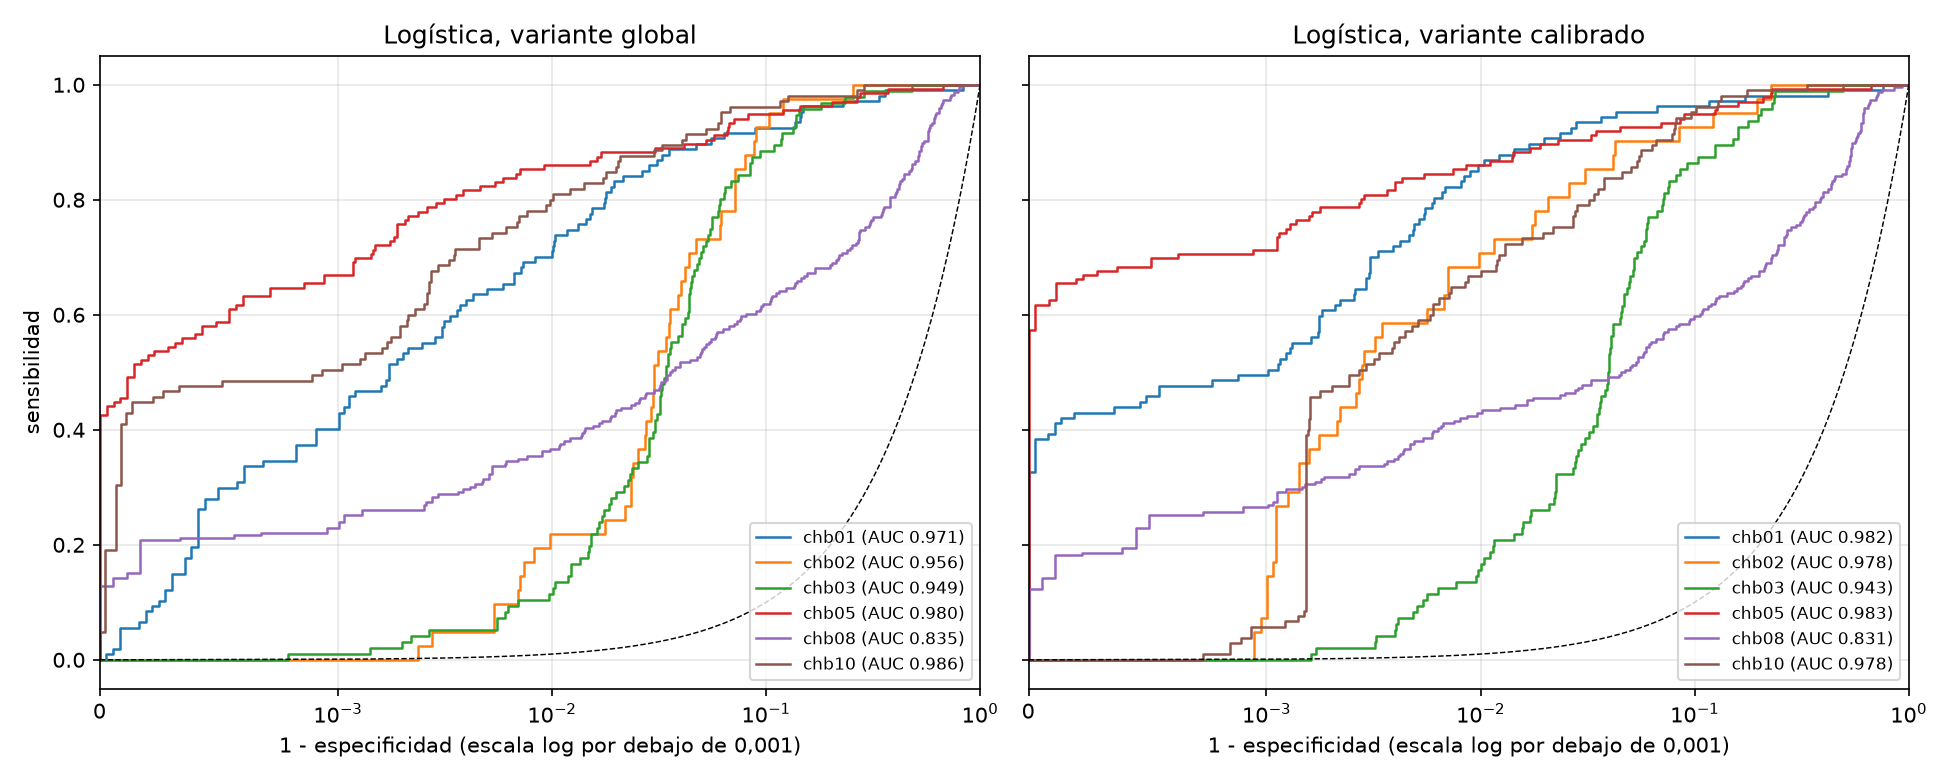
\includegraphics[width=\textwidth]{etapa3/chbmit_lopo_roc.png}
  \caption{CHB-MIT, LOPO: curvas ROC de la regresión logística por paciente de prueba, sin calibrar (izquierda) y
           calibrada (derecha). Eje horizontal lineal entre 0 y $10^{-3}$ y logarítmico por encima.}
  \label{fig:lopo_roc}
\end{figure}

Las curvas ROC por paciente (Figura~\ref{fig:lopo_roc}) muestran por qué el AUC no alcanza:
\begin{itemize}
  \item \textbf{chb03} tiene AUC 0,95, pero con menos de 1~\% de falsos positivos casi no detecta nada: sus ventanas con
        mayor puntaje no son crisis. Es el paciente más difícil en la zona útil, también para la CNN.
  \item \textbf{chb05 y chb10} detectan la mitad de las ventanas ictales con menos de 0,1~\% de falsos positivos.
  \item \textbf{chb08} tiene el menor AUC (0,83): sus crisis son las más largas y las de menor aumento de potencia
        (Tabla~\ref{tab:dif_log}). Aun así, se detectan sus 5 crisis, porque al ser largas basta con acertar algunas
        ventanas de cada una.
  \item \textbf{Calibrar} mejora mucho la zona de baja tasa de falsos positivos en chb01 y chb05.
\end{itemize}

\begin{figure}[ht]
  \centering
  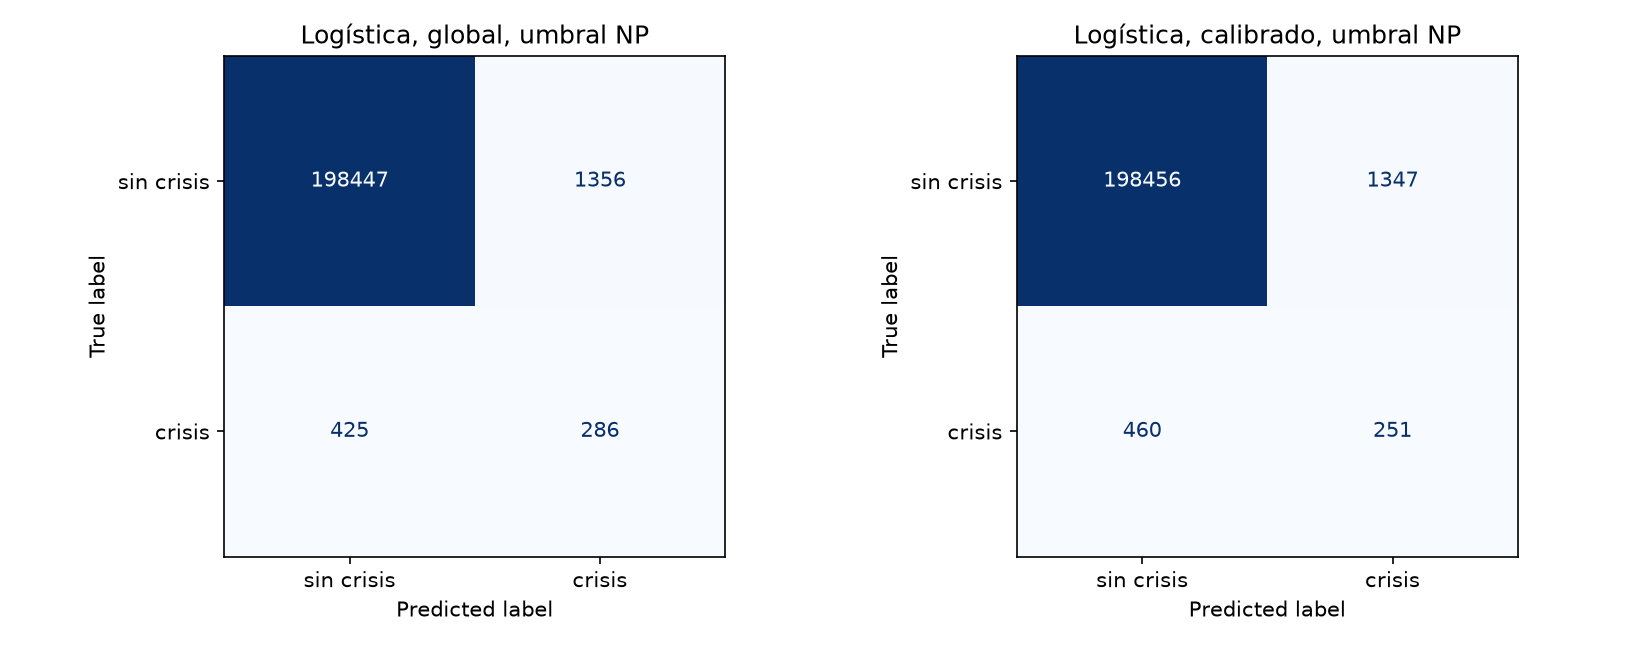
\includegraphics[width=0.85\textwidth]{etapa3/chbmit_lopo_confusion.png}
  \caption{CHB-MIT, LOPO: matrices de confusión por ventana sumadas sobre los 6 pacientes de prueba (regresión logística,
           umbral de Neyman-Pearson, sin ventanas de borde).}
  \label{fig:lopo_confusion}
\end{figure}

La matriz de confusión agregada de la variante calibrada (Figura~\ref{fig:lopo_confusion}) tiene 251 verdaderos positivos,
460 falsos negativos, 1347 falsos positivos y 198\,456 verdaderos negativos. Hay más falsos positivos que ventanas ictales
en total: por~\eqref{eq:vpp_bayes}, el VPP por ventana es apenas $251/1598 = 0{,}16$. Por evento el panorama es mejor,
porque los falsos positivos se agrupan en rachas y las crisis duran varias ventanas.

\section{Resultados en CHB-MIT: partición fija}
\label{sec:fija_convexos}

Para comparar con la CNN, los modelos convexos se evalúan también con la partición fija de la Tabla~\ref{tab:particion}:
entrenamiento con chb02, chb05 y chb08, umbral de Neyman-Pearson calculado con las ventanas sin crisis de chb01, y prueba
en chb03 y chb10.

\begin{table}[ht]
\centering
\caption{CHB-MIT, partición fija. Prueba: chb03 y chb10 (14 crisis, 87,8 horas sin crisis).}
\label{tab:fija_convexos}
\begin{tabular}{llcccccc}
\toprule
Variante & Modelo & AUC val. & AUC prueba & Sens. & Crisis & FA/h & Lat. [s] \\
\midrule
global    & logística  & 0,969 & 0,799 & 0,304 & 5/14 & 3,26 & 14,0 \\
global    & SVM lineal & 0,967 & 0,798 & 0,304 & 7/14 & 2,94 & 18,0 \\
calibrado & logística  & 0,979 & \textbf{0,934} & 0,269 & 7/14 & 1,22 & 26,0 \\
calibrado & SVM lineal & 0,977 & 0,930 & 0,244 & 6/14 & \textbf{1,00} & 24,5 \\
\bottomrule
\end{tabular}
\end{table}

Con solo tres pacientes de entrenamiento, la variante global generaliza mal: AUC de 0,97 en validación pero 0,80 en
prueba. La calibrada llega a 0,93 en prueba y reduce las falsas alarmas de 3,3 a 1,2 por hora (Tabla~\ref{tab:fija_convexos}).
Detecta la mitad de las crisis, con una latencia mediana de 26~s. La regresión logística calibrada es la línea de base contra
la que se compara la CNN en el Capítulo~\ref{cap:resultados}.
